% Copyright 2024 the authors. All rights reserved.

% Style Notes
% -----------
% - USE mdframed BOXES FOR IMPORTANT RESULTS!
% - Use $d\plus1$ for an in-text or wordy d+1, and $d+1$ for an in-equation or mathy $d+1$.
% - Don't put hyphens in timelike, spacelike, lightlike (null).
% - Typeset d-vectors and (d+1)-vectors using the macros, not by hand.
% - Use "~~" sparingly to make large separations in an equation but almost always use "~".
% - Use \metric and \proj and everything else we have defined.
% - We call it "orthonormalization" not "orthogonalization".
% - Use bras and kets only for unit vectors in d+1.
% - It's a Lorentz transform or a transformation operator. Audit!

% To-do
% -----
% - Change the plotting so there are no more PRIMES. We use u and v, not primes.
% - Should we shorten Lorentz transform to LT?
% - Stronger literature searches.
% - This paper is relevant, maybe? https://arxiv.org/abs/1103.1072
% - The references are a mess: German or English titles? Order? arXiv entries? Make it not suck.
% - Should we prove things? SOLE, do you have opinions? HOGG would love to put in some Definitions, Proofs, and Lemmas!
% - Search for all HOGG, SOLE, \cite{} and fix them.
% - This paper is too long! It only says a few things. Try to tighten it up.
% - Where to submit? Maybe European Journal of Physics? (Open Access) or American Journal of Physics? (Maybe higher impact?)

\documentclass{article}
\usepackage[utf8]{inputenc}

% linx
\usepackage[hidelinks]{hyperref}

% math definitions
\newcommand{\metric}{\mathsf{H}}
\newcommand{\proj}{\mathsf{\Pi}}
\usepackage{amsmath,amsfonts,mathrsfs}
\DeclareMathOperator{\dd}{d\!}
\newcommand\upvec[1]{\!\vec{\,\mathrm{#1}}}
\newcommand{\Evec}[1]{{\mathbf{#1}}} % d-vector
\newcommand{\Ehat}[1]{{\mathbf{\hat{#1}}}} % d-vector unit vector
\newcommand{\Lvec}[1]{\upvec{\mathsf{#1}}} % (d+1)-vector
\newcommand{\Lhat}[1]{\hat{\mathsf{#1}}} % (d+1)-vector unit vector
\newcommand{\Lblank}[1]{\mathsf{#1}} % (d+1)-vector unit vector
\newcommand{\bra}[1]{\langle\,{#1}\,|}
\newcommand{\ket}[1]{|\,{#1}\,\rangle}
\newcommand{\braket}[2]{\langle\,{#1}\,|\,{#2}\,\rangle}
\newcommand{\ketbra}[2]{|\,{#1}\,\rangle\,\langle\,{#2}\,|}
\newcommand{\plus}{\!+\!} % evil

% fixing latex page layout and typography
\usepackage[letterpaper]{geometry}
\setlength{\textwidth}{5.50in}
\setlength{\textheight}{9.40in}
\setlength{\oddsidemargin}{3.25in}
\addtolength{\oddsidemargin}{-0.5\textwidth}
\setlength{\topmargin}{-0.55in}
\renewcommand{\small}{\normalsize} % pure evil
\linespread{1.08}
\frenchspacing\raggedbottom\sloppy\sloppypar
\pagestyle{myheadings}
\markboth{}{\textsf{Hogg \& Villar / Relativistic orthonormalization and coordinate-free boost transforms}}
\newcommand{\documentname}{\textsl{Note}}
\newcommand{\secref}[1]{Section~\ref{#1}}
\newcommand{\figref}[1]{Figure~\ref{#1}}

% figure boxes and figure layout
\usepackage{graphicx}
\graphicspath{{./notebooks/}}
\usepackage[framemethod=tikz]{mdframed}
\usetikzlibrary{shadows}
\definecolor{captiongray}{HTML}{555555}
\mdfsetup{%
  innertopmargin=2ex,
  innerbottommargin=1.8ex,
  linecolor=captiongray,
  linewidth=0.5pt,
  roundcorner=1pt,
  shadow=false,
  %shadowcolor=black!05,
  %hadowsize=4pt
}
\newlength{\figurewidth}
\setlength{\figurewidth}{0.315\textwidth}
\setlength{\floatsep}{1ex}
\setlength{\textfloatsep}{1ex}

% delete me:
\usepackage{xcolor}
\newcommand{\SOLE}[1]{\textcolor{purple}{\textsl{SOLE says: {#1}}}}
\newcommand{\HOGG}[1]{\textcolor{violet}{\textsl{HOGG says: {#1}}}}

\title{\bfseries Relativistic orthonormalization and coordinate-free Lorentz transforms}
\author{\textbf{David W. Hogg}\footnote{DWH is in the Center for Cosmology and Particle Physics, Department of Physics, New York University, and in the Max Planck Institute for Astronomy, and in the Center for Computational Astrophysics, Flatiron Institute. Send email to \texttt{<david.hogg@nyu.edu>}.}
        \and
        \textbf{Soledad Villar}\footnote{SV is in the Department of Applied Mathematics and Statistics, Johns Hopkins University, and in the Mathematical Institute of Data Science, Johns Hopkins University, and in the Center for Computational Mathematics, Flatiron Institute.}}
\date{draft as of 2024 August 21}

\begin{document}\thispagestyle{plain}
\maketitle

\begin{abstract}\noindent
    Special and general relativity in $d\plus1$ spacetime dimensions (our macroscopic Universe is $3\plus1$) can be thought of as metric theories with a metric that isn't positive definite, such that timelike, spacelike, and lightlike (null) vectors have positive, negative, and zero magnitudes.
    These spacetimes violate of a lot of the intuitions we have about subspaces, inner products, and orthogonality.
    The concept of orthonormalization (Gram--Schmidt, for example) carries over to Lorentz space (Minkowski space), but there are pathologies in which it is possible for the procedure to produce a lightlike vector and thus bork.
    We describe how to avoid this and successfully orthonormalize any $d+1$ linearly independent input vectors; every successful such orthonormalization produces one timelike and $d$ spacelike unit vectors, all orthogonal (in the Lorentz sense).
    We use this orthonormalization to construct coordinate-free representations of Lorentz transforms that fix or align particular vectors or subspaces.
    That is, we effectively present \emph{a new parameterization of all possible Lorentz transforms} for all $d\plus1$ spacetimes (or even $d\plus s$).
\end{abstract}

\section{Introduction}\label{sec:intro}

Special relativity \cite{sr} is a purely kinematic theory, which can be formulated in terms of vector displacements between \emph{events}.
These vector displacements are 4-vectors in $(3\plus1)$-dimensional spacetime, which has three spatial dimensions and one time dimension.
The coordinate system can be varied not just by rotations and translations, but also by \emph{boosts}, in which the stationary observer (or equivalently the zero-point of 3-vector velocity) is redefined.
Most of the remarkable and counter-intuitive aspects of special relativity---time dilation, length contraction, twin paradox, and so on---flow from the fact that boost transformations preserve not the usual vector magnitudes and inner products, but instead magnitudes and inner products made with a \emph{non-positive-definite metric tensor}\footnote{For some, you can't call something a ``metric tensor'' if it isn't positive definite: How can you use a metric to define displacements if those displacements won't satisfy the triangle inequality? But that's where we are.}.
General relativity~\cite{gr} is a dynamical theory in which the non-positive-definite spacetime metric becomes (in general) a function of space and time, and the resulting curvature of spacetime is related to the energy densities and stresses in the matter and fields.
This \documentname{} is motivated partly by attempts to understand the geometric properties of spacetime with strange metrics---we will focus on special relativity---and to confront a few of the pathologies that arise.

For group theorists, $(3\plus1)$-dimensional special relativity is equivariant with respect to the group called the Lorentz group and denoted O($1,3$).
In ($d\plus1$)-dimensional spacetime the group would be O($1,d$).
The operators in the group O($1,d$) include rotations in the $d$-dimensional spatial subspace of spacetime, reflections in space and time, and boosts.
And then there are groups with \emph{multiple times}, such that it is $(d\plus s)$-dimensional spacetime and the group is O($s,d$).
All these groups are generalizations of the orthogonal group O($d$), which is the group of rotations and reflections in $d$-dimensional space.
In the context of group theory, the word ``equivariant'' means the following:
If you rotate, reflect, or boost the space, all of the predictions of the theory rotate, reflect, and boost appropriately to match.
What group theorists call ``equivariance'', physicists call ``covariance'' or ``symmetry''.

In some sense, the discovery of special relativity was the beginning of the discovery that physics can be stated in a coordinate-free form.
That is, one does not need to specify a coordinate system in order to explain the physical behavior of a system.
Sometimes a coordinate system is useful.
But it is usually not \emph{required}.
In the special-relativity literature, the Lorentz transforms are almost always expressed in a particular coordinate system, aligned with the boost direction (see, eg, \cite{french, zakamska} or just about any other textbook on the subject)
Here we develop completely coordinate-free expressions for these operators in special relativity; our expressions depend on the change of velocity between the two frames, but not on the coordinate system in which this is expressed.

\paragraph{Our contributions:}
In this \documentname, we make two new contributions to the discussion of special relativity:
\begin{itemize}
\item
We deliver (in \secref{sec:orth}) the relativistic (Minkowski or Lorentz or space-time) generalization of Gram--Schmidt orthonormalization.
The only substantive differences between Lorentz orthonormalization and the standard Euclidean orthonormalization are that the inner product of a vector with itself can be negative (!), and that, even if the input vectors are linearly independent, it is possible to get zero-norm vectors after orthonormalization.
Both of these issues flow from the fact that the metric is not positive-definite.
We deliver recommendations to avoid or respond to any zero-norm vectors that appear in the orthonormalization.
\item
We use the output of orthonormalization to produce (in \secref{sec:lt}) a new parameterization or new form for the Lorentz transform, which transforms the coordinates of events between two reference frames.
This new form is coordinate-free, created directly out of the coordinate-basis unit vectors describing the two frames.
It is analogous to the coordinate-free form for a Euclidean rotation matrix, but with modifications to account for the non-positive-definite properties of the metric; it works for all $d\plus s$ spacetimes.
\end{itemize}

\paragraph{Prior work:}
Some of the ideas discussed here have been looked at previously.
In particular, orthonormalization in special relativity is addressed in~\cite{joot}.
However, that previous work does not deal with the pathologies that can arise when orthonormalization is performed on arbitrary collections of vectors.
Coordinate-free Lorentz transforms are developed in~\cite{wagner}, but with a very different notation (in terms of 3-vectors, not 4-vectors) and a very different set of goals (\HOGG{CHECK THIS}).

\section{Review of operations in Euclidean spaces}\label{sec:od}

Before we consider special relativity, it is worth reviewing how an orthonormalization is performed, and how projection and rotation operators are constructed, in ordinary Euclidean space with an ordinary Euclidean metric.
In standard $d$-dimensional space, with the standard Euclidean metric (the identity), containing vectors governed by the standard orthogonal group O($d$), inner products (scalar products) of vectors are defined as follows:
Given two column vectors $\Evec{u},\Evec{v}\in\mathbb{R}^d$ (or, more specifically, $\mathbb{R}^{d\times1}$), the inner product (or scalar product) is defined as
\begin{align}
    \Evec{u}^\top \Evec{v} &= \Evec{v}^\top \Evec{u} ~.
\end{align}
Two vectors $\Evec{u},\Evec{v}$ are considered orthogonal if their inner product vanishes, or $\Evec{u}^\top\Evec{v}=0$.
In Euclidean space, we will call these vectors ``$d$-vectors'' and typeset them bold.

Imagine that we are given a collection of $n\leq d$ linearly independent $d$-vectors $\Evec{v}_1,\Evec{v}_2,\ldots,\Evec{v}_n$,
and we want to construct orthonormal basis vectors $\Ehat{u}_1,\Ehat{u}_2,\ldots,\Ehat{u}_n$ that span the linear subspace spanned by the vectors $\Evec{v}_j$.
We can perform this orthonormalization by the Gram--Schmidt process \cite{gramschmidt}:
We sequentially construct orthogonal vectors $\Evec{u}_1,\Evec{u}_2,\ldots,\Evec{u}_n$ and normalize them into orthogonal unit vectors $\Ehat{u}_1,\Ehat{u}_2,\ldots,\Ehat{u}_n$ by the following algorithm:
\begin{align}
    \Evec{u}_1 &\leftarrow \Evec{v}_1 \label{eq:ogs1}
    \\
    \mbox{then for each $j$ ($2\leq j\leq n$) in order:} ~~ \Evec{u}_j &\leftarrow \Evec{v}_j - \sum_{k=1}^{j-1} \frac{\Evec{v}_j^\top\Evec{u}_k}{\Evec{u}_k^\top\Evec{u}_k}\,\Evec{u}_k \label{eq:ogs2}
    \\
    \mbox{then for each $j$ ($1\leq j\leq n$):} ~~ \Ehat{u}_j &\leftarrow \frac{1}{\sqrt{\Evec{u}_j^\top\Evec{u}_j}}\,\Evec{u}_j ~. \label{eq:ogs3}
\end{align}
Note that the procedure in \eqref{eq:ogs2} is order-dependent: If you put the $d$-vectors $\Evec{v}_1,\Evec{v}_2,\ldots,\Evec{v}_n$ into a different order, the orthonormalization will return different specific basis unit vectors $\Ehat{u}_1,\Ehat{u}_2,\ldots,\Ehat{u}_n$.
However, all the different possible returned bases (under permutations of the $\Evec{v}_j$) will span the same $n$-dimentional linear subspace of the $d$-dimentional space.

The reader might be concerned that the orthonormalization involves division by forms like $\sqrt{\Evec{u}^\top\Evec{u}}$.
Provided that the input vectors are nonzero and linearly independent, this divisor will never vanish.
That situation will change when we consider the relativistic case in \secref{sec:orth}.

If you have $n\leq d$ linearly independent $d$-vectors $\Evec{v}_j$ that span an $n$-dimensional subspace $\mathscr{S}$ of the $d$-dimensional space, you can use this orthonormalization procedure to build a subspace projection operator $\proj_\mathscr{S}$
\begin{align}\label{eq:oproj}
    \proj_\mathscr{S} &= \sum_{j=1}^n \Ehat{u}_j\,\Ehat{u}_j^\top ~,
\end{align}
where the $\Ehat{u}_j$ are the orthogonal unit vectors\footnote{Note that because---for us---all vectors $\Evec{u},\Evec{v}$ are column vectors, $\Evec{u}\,\Evec{v}^\top\in\mathbb{R}^{d\times d}$ while $\Evec{u}^\top \Evec{v}\in\mathbb{R}$.} delivered by the orthonormalization procedure applied to the $\Evec{v}_j$.
This projection operator has the property that, for any vector $\Evec{w}\in\mathbb{R}^d$, the vector $\proj_\mathscr{S}\,\Evec{w}$ will lie in the subspace spanned by the $\Evec{v}_j$.
The projection operator $\proj_{\mathscr{S}^\perp}$ into the complementary subspace $\mathscr{S}^\perp$ is then just
\begin{align}\label{eq:oprojcomp}
    \proj_{\mathscr{S}^\perp} &= I_d - \proj_\mathscr{S} ~,
\end{align}
where $I_d$ is the $d\times d$ identity.
One consequence of this line of reasoning is that if you have $n=d$ linearly independent vectors $\Evec{v}_j$, they will span the whole space, and the projection operator $\proj_\mathscr{S}$ will become the identity $I_d$.
That is, if you have an orthonormal basis of $d$ unit vectors $\Ehat{u}_j$, then
\begin{align}\label{eq:oI}
    I_d &= \sum_{j=1}^d \Ehat{u}_j\,\Ehat{u}_j^\top = \sum_{j=1}^d \frac{\Evec{u}_j\,\Evec{u}_j^\top}{\Evec{u}_j^\top\Evec{u}_j} ~,
\end{align}
where we have written it in terms of both the normalized and un-normalized vectors, anticipating results to come.
Physicists might call these forms for $\proj_\mathscr{S}$ and $I_d$ \emph{coordinate-free}:
They are coordinate-free in the sense that they are stated just in terms of the input vectors, not in terms of matrix components.
Or, equivalently, we didn't have to specify my coordinate system when we constructed them; we only had to specify the vectors that span the subspace.

These aren't the only kinds of operators that can be written in this coordinate-free form.
It is also possible to write any rotation--reflection operator $R$ in a coordinate-free form.
First a definition: A matrix $R\in\mathbb{R}^{d\times d}$ is a rotation--reflection operator in the orthogonal group O($d$) if the operator preserves all inner products (scalar products).
That is,
\begin{equation}
    R \in \mbox{O($d$)} ~ \mbox{if and only if} ~ \Evec{u}^\top\Evec{v}=(R\,\Evec{u})^\top(R\,\Evec{v}) ~ \mbox{for all $\Evec{u},\Evec{v}$ in $\mathbb{R}^d$} ~.\label{eq:orth1}
\end{equation}
This, in turn, will be true if and only if $R$ is a square root of the identity:
\begin{equation}
    R \in \mbox{O($d$)} ~ \mbox{if and only if} ~ R^\top R=I_d ~.\label{eq:orth2}
\end{equation}
We call $R$ a rotation--reflection operator because the group encompasses all rotations, all reflections, and all combinations of rotations and reflections.

For example, the simplest (interesting) orthogonal space is O($2$). In this case the operators form a one-dimensional family; they are all of the form
\begin{align}
    R &= \begin{bmatrix}\cos{\theta} & -\sin{\theta} \\ \sin{\theta} & \cos{\theta}\end{bmatrix} ~\mbox{or}~
    \begin{bmatrix}-\cos{\theta} & \sin{\theta} \\ \sin{\theta} & \cos{\theta}\end{bmatrix} \label{eq:o2}
    \\
    -\pi &< \theta < \pi ~, \nonumber
\end{align}
where $\theta$ is a rotation angle.
The two choices in \eqref{eq:o2} correspond to, in one case, pure rotation and, in the other, rotation plus reflection.
When $d>2$ the coordinate representations of the $R$ become large matrices full of trig functions.
They get very complicated, while the coordinate-free representations we are about to deliver stay simple.

Now how do we construct general coordinate-free forms for the operators $R$?
Usually they are given in terms of sines and cosines of rotation angles, plus sign flips, as they are in \eqref{eq:o2}.
However, there are coordinate-free forms.
For example: Imagine that we have two complete orthonormal bases in $\mathbb{R}^d$, $\Ehat{u}_1,\Ehat{u}_2,\ldots,\Ehat{u}_d$ and $\Ehat{v}_1,\Ehat{v}_2,\ldots,\Ehat{v}_d$.
We can now imagine a rotation--reflection operator $R$ that rotates and reflects any $d$-vector $\Evec{w}$ in the same way that these two bases are rotated and reflected with respect to one another.
This particular operator $R$ can be constructed by the following coordinate-free outer-product construction:
\begin{align}
    R &= \sum_{j=1}^d \Ehat{v}_j\,\Ehat{u}_j^\top ~.\label{eq:rotationoperator}
\end{align}
That is, rotations and reflections can be specified directly using orthonormal bases, with no explicit reference to any angles or coordinates.
In this sense, this form could be thought of as a ``vector-guided'' rotation matrix:
It is constructed directly from the vectors, and independent of how those vectors are represented.
It is therefore coordinate-free.
In case it is unfamiliar, this form \eqref{eq:rotationoperator} for transformation operators is advocated for and used in, eg, \HOGG{Sole can you help here? I can't find any clear textbook use of this form for the rotation operator. If this is novel, which it most certainly is not, then we can prove something here?}

Finally, there is an even simpler expression for the rotation operator $R$ that rotates a vector through the angle betweeen unit vector $\Ehat{u}$ and unit vector $\Ehat{v}$ in the plane defined by $\Ehat{u}$ and $\Ehat{v}$; that is, the minimal rotation operator that takes $\Ehat{u}$ to $\Ehat{v}$.
This is
\begin{align}
    R &= \Ehat{v}\,\Ehat{u}^\top - \Ehat{u}\,\Ehat{v}^\top + (\Ehat{u}^\top\Ehat{v})\,\proj_{2} + \proj_{d-2} \label{eq:vecs2rot} \\
    \proj_2 &= \frac{[\Ehat{u}\,\Ehat{u}^\top + \Ehat{v}\,\Ehat{v}^\top] - (\Ehat{u}^\top\Ehat{v})\,[\Ehat{u}\,\Ehat{v}^\top + \Ehat{v}\,\Ehat{u}^\top]}{1 - (\Ehat{u}^\top\Ehat{v})^2} ~,
\end{align}
where $\proj_2$ is the projection operator that projects onto the subspace spanned by $\Ehat{u}$ and $\Ehat{v}$, and $\proj_{d-2} = I_d - \proj_2$ is the complementary projection operator.
This is a useful expression when you aren't given two complete coordinate bases, but instead just the two directions that define the endpoints of the rotation; it will be very useful in the relativistic case below.

\begin{figure}[t]
\begin{mdframed}
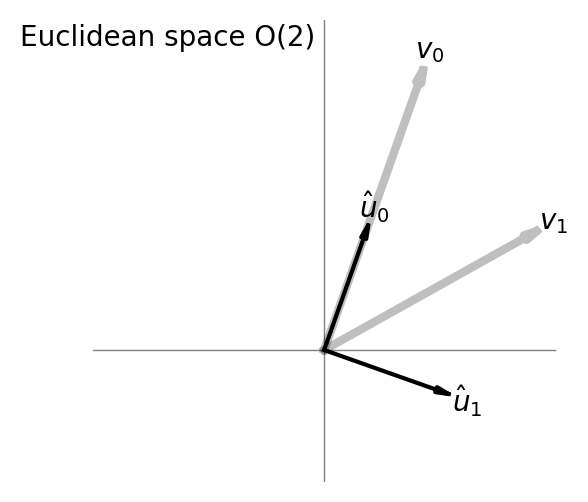
\includegraphics[width=\figurewidth]{E_v.png}%
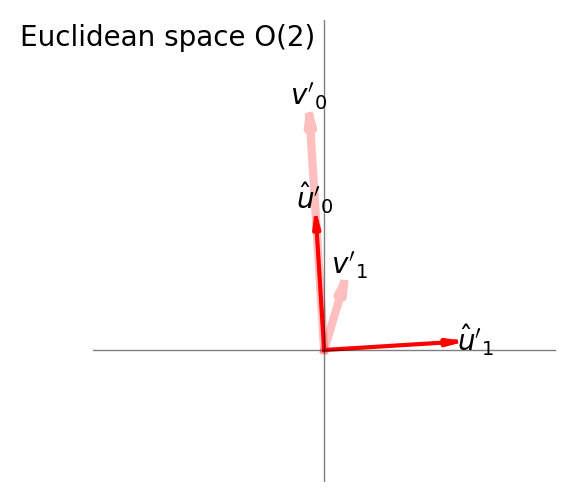
\includegraphics[width=\figurewidth]{E_vp.png}%
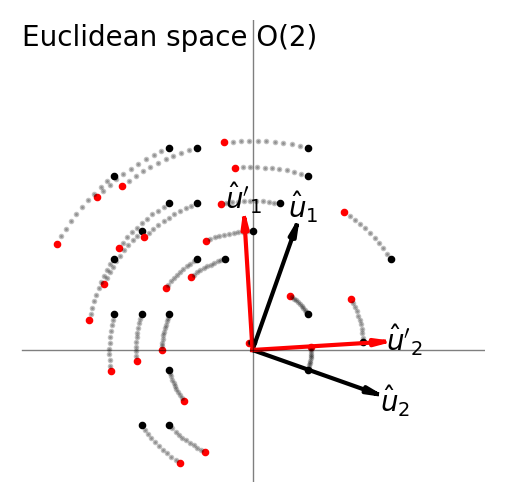
\includegraphics[width=\figurewidth]{E_Q.png}
\caption{A demonstration of orthonormalization and rotation in Euclidean 2-dimensional space O($2$).
    \textsl{Left:} Two 2-vectors $\Evec{v}_1, \Evec{v}_2$ and the corresponding orthonormal 2-vectors $\Ehat{u}_1, \Ehat{u}_2$ obtained by the orthonormalization procedure.
\textsl{Middle:} A different two vectors $\Evec{v}'_1, \Evec{v}'_2$ and the corresponding orthonormal vectors $\Ehat{u}'_1, \Ehat{u}'_2$.
\textsl{Right:} The action of the rotation operator $R$ generated from the orthonomal pairs $\Ehat{u}_1, \Ehat{u}_2$ and $\Ehat{u}'_1, \Ehat{u}'_2$.
The black points rotate to the red points under the action of the operator $R$.
The grey points in between are presented to guide the eye.\label{fig:Euclid}}
\end{mdframed}
\end{figure}
The result of orthonormalization of two pairs of 2-vectors in O($2$) ($d=2$) is shown in \figref{fig:Euclid}.
Also shown in \figref{fig:Euclid} is the action of the rotation operator $R$ derived from the basis vectors generated by those two orthonormalizations.

\section{Relativistic notation and transformations}\label{sec:notation}

There is a history of notation in special and general relativity.
Here we deliver a translation from traditional Einstein summation notation, and traditional language about boost, to a more linear-algebra-oriented notation.
After this Section, we will be using exclusively the linear-algebra notation, which is simpler (for us).

In Lorentz or Minkowski space, we think of there being a metric $\metric$ (often called $g^{\mu\nu}$ or $\eta^{\mu\nu}$ or $\eta$), which is a $(d\plus1)\times(d\plus1)$ matrix that is \emph{not} positive definite.
The metric $\metric$ is diagonal with $+1$ in the first position and $-1$ repeated on all the remaining $d$ diagonal elements.
In $3\plus1$ this is
\begin{align}\label{eq:sig}
    \metric &= \begin{bmatrix}1 & 0 & 0 & 0\\
                              0 & -1 & 0 & 0\\
                              0 & 0 & -1 & 0\\
                              0 & 0 & 0 & -1\end{bmatrix} ~.
\end{align}
There is another possible signature---with $-1$ in the first position and $+1$ thereafter.
In this \documentname{} we choose the signature illustrated in \eqref{eq:sig}; nothing significant in our discussion changes if you choose the opposite signature.
Indeed, this is one of the main reasons to pursue a coordinate-free formulation of special relativity:
The coordinate-free representations don't care about the signature of your metric, or any other aspects of your coordinate system.\footnote{It is precisely because the choice of signature doesn't matter that physicists will constantly argue about it. We don't know many physicists who don't have a strong opinion about the signature. We ourselves have no strong opinion, and our expressions are agnostic to the signature.}
The signature of the metric will only come up in our definitions of ``timelike'' \eqref{eq:timelike}, ``lightlike'' \eqref{eq:lightlike}, and ``spacelike'' \eqref{eq:spacelike} below.

The metric we have described is the metric for $d\plus 1$ spacetime.
In $d\plus s$ the diagonal of the metric has $s$ values set to $+1$ and $d$ values set to $-1$ (or the opposite for the opposite signature).

We are going to consider vectors $\Lvec{u}, \Lvec{v}, \Lvec{w}\in\mathbb{R}^{(d+1)}$ in Lorentz space or Minkowski space or spacetime.
We will call these vectors ``($d\plus1$)-vectors'', and typeset them sanserif with hats (arrows or carets, depending).

Old-school relativists tend to write the relativistic inner product (the scalar product or Minkowski inner product) between two ($d\plus1$)-vectors $\Lvec{u}$ and $\Lvec{v}$ as
\begin{align}
    \Lblank{u}^\mu\,\Lblank{v}_\mu &= \Lblank{v}^\mu\,\Lblank{u}_\mu ~,
\end{align}
where $\mu$ is a component index (such that $\Lblank{u}_\mu$ is the $\mu$th component of $\Lvec{u}$) with $1\leq\mu\leq d+1$, and the repeated index is (implicitly) summed\footnote{%
In these expressions, greek indexes like $\mu$, $\nu$ are be indexes over vector components (going from 1 to 4 in $3\plus1$, for example), and (later) roman indexes like $i$, $j$, $k$ will be indexes over vectors or other things.} .
The $\Lblank{u}^\mu$ is a contravariant vector component and the $\Lblank{v}_\mu$ is a covariant vector component.
Contravariant and covariant components are related as follows:
\begin{align}
    \Lblank{u}^\mu &= \metric^{\mu\nu}\,\Lblank{u}_\nu \equiv \sum_{\nu=1}^{d+1} \metric^{\mu\nu}\,\Lblank{u}_\nu
    \\
    \Lblank{u}^\mu\,\Lblank{v}_\mu &= \metric^{\mu\nu}\,\Lblank{u}_\mu\,\Lblank{v}_\nu \equiv \sum_{\mu=1}^{d+1}\sum_{\nu=1}^{d+1} \metric^{\mu\nu}\,\Lblank{u}_\mu\,\Lblank{v}_\nu
\end{align}
where the $\metric^{\mu\nu}$ are the components of the metric $\metric$.
The implicit summations on the left of the ``$\equiv$'' signs are guided by the rules of what's called Einstein summation notation (\cite{summation}; it is a subset of the Ricci calculus~\cite{ricci}): Indexes can appear exactly once or exactly twice (and no more) and when they appear twice, one must be up and one must be down, and they are summed from 1 to $d+1$.

In linear algebra notation, if we think of $\Lvec{u}$ and $\Lvec{v}$ as being column vectors in $\mathbb{R}^{d+1}$ (or, to be extremely specific, $\mathbb{R}^{(d+1)\times 1}$), then we can write this same inner product as
\begin{align}\label{eq:inner}
    \Lvec{u}^\top\metric\,\Lvec{v} &= \Lvec{v}^\top\metric\,\Lvec{u} ~.
\end{align}
We are going to use this notation going forward, not the Einstein summation notation.

What, physically, are the ($d\plus1$)-vectors of special relativity?
Events in spacetime are represented by one time coordinate and three spatial coordinates (a position); they are things that happened at some place and time.
The displacement $\Lvec{s}$ between two events is a ($d\plus1$)-vector.
In $d\plus1$ spacetime there are generalizations of many standard $d$-vectors to which you are accustomed.
For example,
the ($d\plus1$)-vector velocity $\Lvec{u}$ is a timelike vector with $\Lvec{u}^\top\metric\,\Lvec{u}=1$ (a unit vector), where the spatial part of $\Lvec{u}$ (the last $d$ components) is proportional to what is traditionally the $d$-vector velocity.
In $d=3$ spatial dimensions the ($3\plus1$)-vector velocity $\Lvec{u}$ is given by
\begin{align}
    \Lvec{u}^\top &= \begin{bmatrix} \gamma & \gamma\,\beta_x & \gamma\,\beta_y & \gamma\,\beta_z \end{bmatrix} \\
    \gamma &= (1 - \beta_x^2 - \beta_y^2 - \beta_z^2)^{-1/2} \nonumber\\
    \begin{bmatrix} \beta_x & \beta_y & \beta_z\end{bmatrix} &= \begin{bmatrix}\displaystyle\frac{1}{c}\,\frac{\dd x}{\dd t} & \displaystyle\frac{1}{c}\,\frac{\dd y}{\dd t} & \displaystyle\frac{1}{c}\,\frac{\dd z}{\dd t} \end{bmatrix} = \frac{1}{c}\,\Evec{v}^\top ~,\nonumber
\end{align}
where the transpose on $\Lvec{u}$ is a reminder that ($d\plus1$)-vectors are really column vectors,
$c$ is the speed of light in a vacuum (or the speed of lightlike or null trajectories),
and the $\beta_k$ are the components of a dimensionless 3-vector velocity $\Evec{v}/c$.
Explicit calculation demonstrates that $\Lvec{u}^\top\metric\,\Lvec{u}=1$ for all settings of $\Evec{v}/c$.
Another ($d\plus1$)-vector example is the ($d\plus1$)-vector momentum $\Lvec{p}$ of a particle.
This is a timelike vector with $\Lvec{p}^\top\metric\,\Lvec{p}=m^2\,c^4$, where $m$ is the rest mass of the particle.
The ($d\plus1$)-vector momentum has the energy $E / c$ of the particle as its first component (the time component), and the Euclidean $d$-vector momentum $\Evec{p}$ in its remaining $d$ components.\footnote{%
If you write out the inner product $\Lvec{p}^\top\metric\,\Lvec{p}$ for the ($d\plus1$)-vector momentum $\Lvec{p}$, you get $$E^2 - \Evec{p}^\top\Evec{p}\,c^2 = m^2\,c^4~,$$ where $\Evec{p}$ is the $d$-vector (spatial) momentum. In the rest frame, this becomes $E=m\,c^2$. This is the equation that made Einstein famous.}

When you change reference frames, a Lorentz transform is applied.
Under the Lorentz transform, the components of all of the ($d\plus1$)-vectors will change, but all the inner products among them (and with themselves) will remain the same.

In standard special-relativity lore, Lorentz transforms are taught as \emph{boost transforms} in which the assignment of the stationary observer is changed and the time and space axes change accordingly.
For our purposes, the Lorentz transforms also include spatial rotations, spatial reflections, and even time reflections (gasp!):
That is, for our purposes, an operator $Q$ is a valid Lorentz transform if it is a member of the Lorentz group O($1,d$).
To be more specific, an operator $Q$ (which can be thought of as a $(d+1)\times(d+1)$ matrix) is a Lorentz transform---is an operator in the group O($1,d$)---if it preserves all inner products (scalar products). 
That is,
\begin{equation}
    Q \in \mbox{O($1,d$)} ~ \mbox{if and only if} ~ \Lvec{u}^\top\metric\,\Lvec{v}=(Q\,\Lvec{u})^\top\metric\,(Q\,\Lvec{v}) ~ \mbox{for all $\Lvec{u},\Lvec{v}$ in $\mathbb{R}^{d+1}$} ~.\label{eq:lore1}
\end{equation}
This, in turn, will be true if and only if $Q$ leaves the metric unchanged:
\begin{equation}
    Q \in \mbox{O($1,d$)} ~ \mbox{if and only if} ~ Q^\top\metric\,Q=\metric ~.\label{eq:lore2}
\end{equation}
This is our (surprising, perhaps) definition of the Lorentz transform $Q$.
Note how similar the Lorentz-group statements \eqref{eq:lore1} and \eqref{eq:lore2} are to the orthogonal-group statements \eqref{eq:orth1} and \eqref{eq:orth2}.
In a sense, group elements $Q$ are square roots of the metric $\metric$.

For example, the simplest non-trivial Lorentz space is O($1,1$) or $1\plus1$ ($d=1$).
In this case, the Lorentz transforms form a one-dimensional family; they are all of the form
\begin{align}
    Q &= \begin{bmatrix}\gamma & \beta\,\gamma \\ \beta\,\gamma & \gamma\end{bmatrix} ~\mbox{or}~
    \begin{bmatrix}-\gamma & -\beta\,\gamma \\ \beta\,\gamma & \gamma\end{bmatrix} ~\mbox{or}~
    \begin{bmatrix}\gamma & \beta\,\gamma \\ -\beta\,\gamma & -\gamma\end{bmatrix}  ~\mbox{or}~
    \begin{bmatrix}-\gamma & -\beta\,\gamma \\ -\beta\,\gamma & -\gamma\end{bmatrix} \label{eq:o11}
    \\
    \gamma &\equiv \frac{1}{\sqrt{1 - \beta^2}} ~ \mbox{and} ~ -1 < \beta < 1 ~.\nonumber
\end{align}
In this simple case, $\beta$ is the dimensionless velocity of the boost, and $\gamma$ is the Lorentz factor.
The four choices in \eqref{eq:o11} correspond to even parity, reversing time, reversing space, and reversing both.\footnote{%
Many physicists would not permit reversals of time or space among the Lorentz transforms.
These reversals appear inevitably when we define the set of Lorentz transforms to be all the operators $Q$ such that $\metric=Q^\top\metric\,Q$, as we do.
So we depart here slightly from standard practice by being maximally inclusive.}
But in what follows we are going to develop \emph{coordinate-free forms} for the Lorentz transforms, in analogy to the coordinate-free forms for the rotation--reflection operators given in \secref{sec:od}.

Finally we remark that---because the metric is non-positive-definite---a nonzero ($d\plus1$)-vector $\Lvec{v}$ can come in three forms, \emph{timelike}, \emph{spacelike}, or \emph{lightlike} (sometimes \emph{null}):
\begin{align}
    \Lvec{v} ~ \mbox{is timelike}  &~ \mbox{if} ~ \Lvec{v}^\top\metric\,\Lvec{v} > 0 \label{eq:timelike}\\
    \Lvec{v} ~ \mbox{is lightlike} &~ \mbox{if} ~ \Lvec{v}^\top\metric\,\Lvec{v} = 0 \label{eq:lightlike}\\
    \Lvec{v} ~ \mbox{is spacelike} &~ \mbox{if} ~ \Lvec{v}^\top\metric\,\Lvec{v} < 0 ~.\label{eq:spacelike}
\end{align}
Technically, these definitions depend on the signature you chose for your metric; you would use the opposite language if you chose the opposite signature.
This is the only point in this \documentname{} that depends on the signature; everything else is agnostic to signature.
Because Lorentz transforms $Q\in$~O($1,d$) preserve inner products, you can't Lorentz transform a vector from any one of these three categories (timelike, lightlike, or spacelike) to any other of these categories; the category (timelike, lightlike, or spacelike) is a Lorentz invariant property of the ($d\plus1$)-vector.

\section{Relativistic orthonormalization}\label{sec:orth}

In Lorentz space we will still say that two ($d\plus1$)-vectors are ``orthogonal'' if their inner product is zero.
\begin{align}
    \Lvec{u},\Lvec{v} ~ \mbox{are orthogonal if and only if} ~ \Lvec{u}^\top\metric\,\Lvec{v}=0 ~,
\end{align}
where the inner product is defined as in \eqref{eq:inner}.
This is great, but it leads to a strange consequence:
Any lightlike vector $\Lvec{v}$ is \emph{orthogonal to itself}.
This is just one aspect of the oddness of orthogonality under the Lorentz metric:
It is also the case that orthogonal vectors aren't generally at 90 degrees with respect to each other; in fact angles aren't obviously defined for general ($d\plus1$)-vectors in spacetime.
As for normalized, we will say that a ($d\plus1$)-vector is ``normalized'' or is a ``unit'' vector (and typeset it with a hat like $\Lhat{u}$ or $\Lhat{v}$) if the inner product with itself $\Lhat{u}^\top\metric\,\Lhat{u}$ is either $+1$ or $-1$.
\begin{align}
    \Lvec{u} ~ \mbox{is normalized if and only if} ~ |\Lvec{u}^\top\metric\,\Lvec{u}| = 1 ~.
\end{align}
Note that lightlike vectors cannot be normalized.

We will still have linear dependence and independence exactly as in Euclidean space.
That is, $n$ ($d\plus1$)-vectors $\Lvec{v}_j$ are linearly independent if there is no non-trivial set of $n$ coefficients $a_j\in\mathbb{R}$ such that $\sum_{j=1}^n a_j\,\Lvec{v}_j = 0$.

How does orthonormalization work in relativity?
Start with $n\leq d+1$ linearly independent ($d\plus1$)-vectors $\Lvec{v}_1,\Lvec{v}_2,\ldots,\Lvec{v}_n$.
If these vectors are randomly generated, then with high probability the straightforward generalization of Gram--Schmidt will work:
\begin{align}
    \Lvec{u}_1 &\leftarrow \Lvec{v}_1 \label{eq:rgs1}
    \\
    \mbox{then for each $j$ ($2\leq j\leq n$) in order:} ~~ \Lvec{u}_j &\leftarrow \Lvec{v}_j - \sum_{k=1}^{j-1} \frac{\Lvec{v}_j^\top\metric\,\Lvec{u}_k}{\Lvec{u}_k^\top\metric\,\Lvec{u}_k}\,\Lvec{u}_k \label{eq:rgs2}
    \\
    \mbox{then for each $j$ ($1\leq j\leq n$):} ~~ \Lhat{u}_j &\leftarrow \frac{1}{\sqrt{|\Lvec{u}_j^\top\metric\,\Lvec{u}_j|}}\,\Lvec{u}_j ~, \label{eq:rgs3}
\end{align}
where we had to insert an absolute value inside the square-root operation because negative inner products will appear.
We're done. \emph{Ta-da!}
But we aren't really done, because the iteration step \eqref{eq:rgs2} involves dividing by an inner product, and inner products can vanish if the procedure accidentally produces a lightlike vector $\Lvec{u}_j$ for some $j$.

In principle (and in practice if your context is adversarial), the orthonormalization procedure in \eqref{eq:rgs2} can produce a lightlike vector.
If you start with $n$ linearly independent ($d\plus1$)-vectors $\Lvec{v}_j$, ($1\leq j\leq n$), begin the orthonormalization procedure, and then at some $j$ produce a lightlike $\Lvec{u}_j$, here are the strategies:
\begin{enumerate}
\item If all your input vectors $\Lvec{v}_j$ are lightlike, then by construction, $\Lvec{u}_1$ will be lightlike.
    Replace the first two input vectors $\Lvec{v}_1,\Lvec{v}_2$ with two (possibly randomly constructed) independent linear combinations of the $\Lvec{v}_1$ and $\Lvec{v}_2$.
    Re-start the orthonormalization.
    With high probability the orthonormalization will succeed.
    \item If not every one of your input vectors is lightlike, but the first one is, then by construction ${u}_1$ will be lightlike.
    Reorder the vectors such that the first vector is not lightlike and re-start the orthonormalization.
    With high probability the orthonormalization will succeed.
    \item If none of your input vectors is lightlike, but a lightlike $\Lvec{u}_j$ is appearing, reorder the input vectors and re-start the orthonormalization.
    \item If all of the above fails, replace the $n$ input vectors $\Lvec{v}_j$ with a randomly generated set of $n$ indepdent linear combinations of the original $n$ input vectors.
    With high probability orthonormalization will succeed on this new set of inputs (and, by construction, it will span the same subspace as the original input vectors).
\end{enumerate}
These rules aren't extremely satisfying, because (unless you are extremely careful) they involve changing things like the orientation of the coordinate system.
We conjecture that there are better possible rules.

\HOGG{I think if we start with one timelike first and $n-1$ linearly independent spacelike afterwards, nothing ever borks.
So just do that! Maybe? And can we prove this?}

One comment to make is that orthonormalization is not necessarily numerically stable.
That is, a set of vectors can be formally linearly independent, but only barely, or not at all at finite precision.
It is out of scope for us here, but there are methods to improve the stability of orthonormalizations (\HOGG{SOLE WHAT TO CITE?}); these will be generalizable to the Lorentz space.

Another comment to make is that if you start with $n=d+1$ linearly independent ($d\plus1$)-vectors, the outcome of the orthonormalization will be exactly one timelike vector and exactly $d$ spacelike vectors.
Importantly for what follows, \emph{the algorithm-generated set of normalized unit vectors $\Lhat{u}_1,\Lhat{u}_2,\ldots,\Lhat{u}_{d+1}$ will form a coordinate basis in spacetime}, with one timelike (time) axis unit vector and $d$ orthogonal spacelike (spatial) axis unit vectors.
\HOGG{Sole: Should we prove this?}

Now just like in O($d$) you can use the orthonormalization to make a subspace projection operator.
If you have $n\leq d+1$ linearly independent ($d\plus1$)-vectors that span a subspace $\mathscr{T}$, then you can orthonormalize them and construct the subspace projection operator $\proj_\mathscr{T}$
\begin{align}\label{eq:rproj}
    \proj_\mathscr{T} &= \sum_{j=1}^n \frac{\Lhat{u}_j\,\Lhat{u}_j^\top\metric}{\Lhat{u}_j^\top\metric\,\Lhat{u}_j} = \sum_{j=1}^n \frac{\Lvec{u}_j\,\Lvec{u}_j^\top\metric}{\Lvec{u}_j^\top\metric\,\Lvec{u}_j} ~,
\end{align}
where the $\Lhat{u}_j$ are the orthogonal unit vectors, and the $u_j$ are the un-normalized orthogonal vectors; this differs from the result in \eqref{eq:oproj} in that we have to divide by an inner product $\Lhat{u}_j^\top\metric\,\Lhat{u}_j$ to account for the sign of the inner product, and we have a right multiply of the metric $\metric$.
But notice that \eqref{eq:rproj} reduces to \eqref{eq:oproj} when the metric is the identity (and thus all inner products are positive.
This projection operator has the property that, for any ($d\plus1$)-vector $w$, the vector $\proj_\mathscr{T}\,w$ will lie in the subspace $\mathscr{T}$ spanned by the $n$ original ($d\plus1$)-vectors $v_j$ that were orthonormalized.
Again, the projection operator $\proj_{\mathscr{T}^\perp}$ into the complementary subspace $\mathscr{T}^\perp$ is then just
\begin{align}\label{eq:lprojcomp}
    \proj_{\mathscr{T}^\perp} &= I_{d+1} - \proj_\mathscr{T} ~,
\end{align}
where $I_{d+1}$ is the $(d+1)\times(d+1)$ identity.

If you have a full set of $n=d+1$ linearly independent ($d\plus1$)-vectors $v_j$, they will span the whole ($d\plus1$)-dimensional space, and the projection operator $\proj_\mathscr{T}$ will become the identity $I_{d+1}$.
That is, if you have an orthonormal basis of $d+1$ unit vectors $\Lhat{u}_j$, then
\begin{align}
    I_{d+1} &= \sum_{j=1}^{d+1} \frac{\Lhat{u}_j\,\Lhat{u}_j^\top\metric}{\Lhat{u}_j^\top\metric\,\Lhat{u}_j} = \sum_{j=1}^{d+1} \frac{\Lvec{u}_j\,\Lvec{u}_j^\top\metric}{\Lvec{u}_j^\top\metric\,\Lvec{u}_j} \label{eq:Lidentity} ~,
\end{align}
where we have written it in terms of both the normalized and un-normalized orthogonal vectors; note that $\Lhat{u}_j^\top\metric\,\Lhat{u}_j=\pm 1$.

If your background is quantum mechanics, then you probably use bra--ket and ket--bra notation \cite{dirac}.
For you, an inner product of unit vectors (basis vectors) ought to be written as a bra--ket $\braket{\Lhat{u}}{\Lhat{v}}$, and an outer product of unit vectors ought to be written as a ket--bra $\ketbra{\Lhat{u}}{\Lhat{v}}$.
In quantum-mechanics (braket) notation, a covariant vector (plus some decorations) becomes a bra $\bra{\Lvec{v}}$, and a contravariant vector becomes a ket $\ket{\Lvec{v}}$
\begin{align}
    \ket{\Lhat{u}_j} &\equiv \Lhat{u}_j \label{eq:Lket}\\
    \bra{\Lhat{u}_j} &\equiv \frac{1}{\Lhat{u}_j^\top\metric\,\Lhat{u}_j}\,\Lhat{u}_j^\top\metric ~,\label{eq:Lbra} ~,
\end{align}
where we have taken some liberties in defining the bra $\bra{\Lhat{u}_j}$, and we remind you that $\Lhat{u}_j^\top\metric\,\Lhat{u}_j=\pm 1$.
With these definitions, the expression for the identity \eqref{eq:Lidentity} becomes a standard formula in quantum mechanics:
\begin{align}
    I_{d+1} &= \sum_{j=1}^{d+1} \ketbra{\Lhat{u}_j}{\Lhat{u}_j} \label{eq:LidentityQM} ~.
\end{align}
We'll use this simplifying bra--ket notation below.
Note that even though the inner product $\Lhat{u}^\top\metric\,\Lhat{u}$ can be either $+1$ or $-1$, with these definitions, the bra--ket $\braket{\Lhat{u}}{\Lhat{u}}$ is always $+1$, whether $\Lhat{u}$ is timelike or spacelike.

Because the metric is its own inverse, if we right-multiply by the metric, we make a simple expression for the metric $\metric$ in terms of the basis vectors:
\begin{align}
    \metric &= \sum_{j=1}^{d+1} \frac{\Lhat{u}_j\,\Lhat{u}_j^\top}{\Lhat{u}_j^\top\metric\,\Lhat{u}_j} = \sum_{j=1}^{d+1} \frac{\Lvec{u}_j\,\Lvec{u}_j^\top}{\Lvec{u}_j^\top\metric\,\Lvec{u}_j} ~.
\end{align}
This expression is beautifully independent of the signature of the metric (mentioned in \secref{sec:notation}); it works for either signature.

\section{Vector-guided Lorentz transforms}\label{sec:lt}

All this work with orthonormal ($d\plus1$)-vectors in special relativity is in the service of making a coordinate-free expression for the Lorentz transform.
Consider two observers moving through spacetime.
One (unprime) is moving with ($d\plus1$)-vector velocity $\Lhat{u}$ and the other (prime) is moving with ($d\plus1$)-vector velocity $\Lhat{v}$.
It is a property of any ($d\plus1$)-vector velocity that it is timelike, and we have typeset them as unit vectors because it is also true that any ($d\plus1$)-vector velocity that it has norm 1 (it is a unit vector)
Each of these two observers has a rest frame, and if $\Lhat{u}-\Lhat{v}\neq 0$, those two rest frames are different.
What are the Lorentz transforms between the two frames?
That is, how do I construct transforms $Q\in$~O($1,d$) that boost $\Lhat{u}$ to make it parallel to $\Lhat{v}$, and vice versa?

There are two answers.
The first answer is that one can augment the ($d\plus1$)-vector velocity $\Lhat{u}$ with $d$ additional ($d\plus1$)-vectors $\Lvec{u}_2,\Lvec{u}_3,\ldots,\Lvec{u}_{d+1}$, and we augment the ($d\plus1$)-vector velocity $\Lhat{v}$ with $d$ additional ($d\plus1$)-vectors $\Lvec{v}_2,\Lvec{v}_3,\ldots,\Lvec{v}_{d+1}$.
If you want the Lorentz transform to have no rotation or reflections, you can set $\Lvec{u}_k=\Lvec{v}_k$ for all $k\geq 2$.
Then you orthonormalize the unprimed vectors, with the input order $\Lvec{u},\Lvec{v}_2,\ldots,\Lvec{v}_{d+1}$, to get orthonormal basis vectors $\Lhat{u}_1,\Lhat{u}_2,\ldots,\Lhat{u}_{d+1}$, and you orthonormalize the primed vectors, with the input order $\Lvec{v},\Lvec{v}_2,\ldots,\Lvec{v}_{d+1}$, to get orthonormal basis vectors $\Lhat{v}_1,\Lhat{v}_2,\ldots,\Lhat{v}_{d+1}$.
Armed with these orthonormal basis vectors, the Lorentz transform $Q$ that boosts from the unprimed frame to the primed frame is simply
\begin{mdframed}
\begin{align}
  Q &= \sum_{j=1}^{d+1} \ketbra{\Lhat{v}_j}{\Lhat{u}_j} ~~ \mbox{iff} ~~ \Lhat{u}_j^\top\metric\,\Lhat{u}_j = \Lhat{v}_j^\top\metric\,\Lhat{v}_j = \pm 1 ~ \mbox{for all $j$} \label{eq:LTQM} ~, \\
  & \tag{\footnotesize Lorentz transform $Q$ given two orthonormal bases $\Lhat{u}_1,\ldots,\Lhat{u}_{d+1}$ and $\Lhat{v}_1,\ldots,\Lhat{v}_{d+1}$}
\end{align}
\end{mdframed}
where we have defined the bras and kets as in \eqref{eq:Lket} and \eqref{eq:Lbra}.
This expression is the relativistic (Lorentz) generalization of the rotation--reflection operator in Euclidean space given in \eqref{eq:rotationoperator}.

A few comments about expression $\eqref{eq:LTQM}$ for the Lorentz transform $Q$ could be the following:
The orthonormalization always returns one timelike and three spacelike vectors;
provided that these are ordered such that they match, that is, provided that $\Lhat{u}_k^\top\metric\,\Lhat{u}_k=\Lhat{v}_k^\top\metric\,\Lhat{v}_k$ for all $k$, the construction of $Q$ given by \eqref{eq:LTQM} will be a valid Lorentz transform.
If the inputs are ordered such that the first input vector ($\Lvec{v}_1$ in the orthonormalization procedure) is timelike, the orthonormalization will make the first output unit vector $\Lhat{u}_1$ be timelike.
If the first input vector is a ($d\plus1$)-vector velocity $\Lhat{u}$ (that is, timelike and unit norm), then the the first output vector $\Lhat{u}_1$ will be identical to the input vector $\Lhat{u}$.
The expression \eqref{eq:LTQM} is coordinate free and independent of the signature choice.
Finally, direct calculation will show that the expression \eqref{eq:LTQM} for $Q$ satisfies the definition \eqref{eq:lore2} of a Lorentz transform.

\begin{figure}[t]
\begin{mdframed}
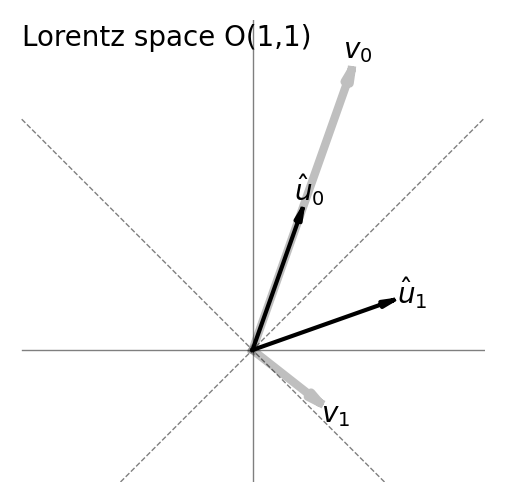
\includegraphics[width=\figurewidth]{L_v.png}%
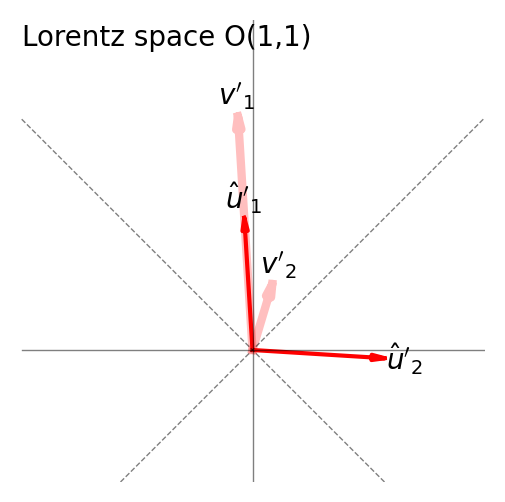
\includegraphics[width=\figurewidth]{L_vp.png}%
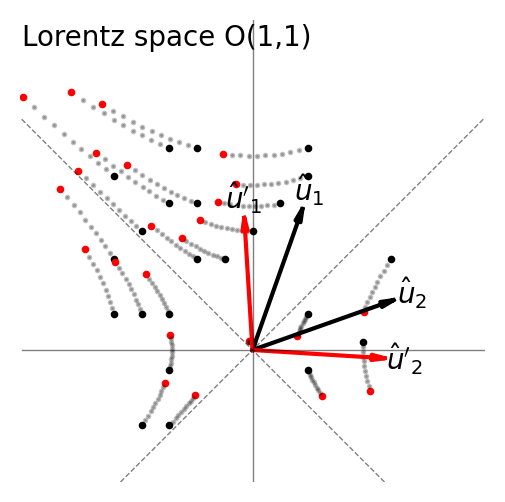
\includegraphics[width=\figurewidth]{L_Q.png}
\caption{A demonstration of orthonormalization and rotation in Lorentz $1\plus1$-dimensional space O($1,1$).
The time coordinate (the first coordinate) is plotted on the vertical axis and the space coordinate (the second coordinate) is plotted on the horizontal axis.
\textsl{Left:} Two ($1\plus1$)-vectors $\Lvec{v}_1, \Lvec{v}_2$ and the corresponding orthonormal vectors $\Lhat{u}_1, \Lhat{u}_2$ obtained by the orthonormalization procedure.
Note that orthonormal vectors in $1\plus1$ neither look orthogonal nor normalized to the eye; the diagonal lightlike (null) lines are plotted to show that orthogonal ($1\plus1$)-vectors are reflected across null lines.
\textsl{Middle:} A different two ($1\plus1$)-vectors $\Lvec{v}'_1, \Lvec{v}'_2$ and the corresponding orthonormal vectors $\Lhat{u}'_1, \Lhat{u}'_2$.
\textsl{Right:} The action of the transform operator (Lorentz transform) $Q$ generated from the orthonormal pairs $\Lhat{u}_1, \Lhat{u}_2$ and $\Lhat{u}'_1, \Lhat{u}'_2$.
The black points transform to the red points under the action of the operator $Q$.
The grey points in between are presented to guide the eye; 
note that they trace out not segments of circles (compare to \figref{fig:Euclid}) but instead segments of hyperbolae.\label{fig:Lorentz}}
\end{mdframed}
\end{figure}
The expression \eqref{eq:LTQM} is a coordinate-free expression for the Lorentz transform, in terms of coordinate basis ($d\plus1$)-vectors.
This is the main contribution of this \documentname.
\figref{fig:Lorentz} illustrates the orthonormalization and the action of the Lorentz transform so constructed in $(1\plus1)$.

In detail, any Lorentz transform can be thought of as being a composition of a boost, a time-reversal, a spatial rotation, and a spatial reflection.
Often when we discuss Lorentz transforms, we want transforms that are boost only.
The procedure above delivers a boost-only transform when the two lists of ($d\plus1$)-vectors to be orthonormalized are identical except for the first elements, which are both timelike.
Spatial rotations and reflections can be introduced by modifying the two lists of ($d\plus1$)-vectors that follow the first (timelike) elements.
The full discussion of all these options is beyond our scope here.

The oddest kind of Lorentz transform is one that reverses the time direction.
We don't recommend making such transforms, but they are permitted here.
These can be constructed by multiplying one of the input ($d\plus1$)-vector velocities (either $\Lvec{u}$ or $\Lvec{u}'$) by $-1$ before starting the orthonormalization.

The second answer to our question---how to construct the Lorentz transform $Q$ starting with two input ($d\plus1$)-vector velocities $\Lhat{u}$ and $\Lhat{v}$---is to write down the minimal Lorentz transform that transforms $\Lhat{u}$ to $\Lhat{v}$.
This is analogous to the rotation matrix expression \eqref{eq:vecs2rot} developed above.
The Lorentz generalization of that expression is the following:
\begin{mdframed}
\begin{align}
    Q &= \ketbra{\Lhat{v}}{\Lhat{u}} - \ketbra{\Lhat{u}}{\Lhat{v}} + \braket{\Lhat{u}}{\Lhat{v}}\,\proj_{1+1} + \proj_{d-1} ~~ \mbox{iff} ~~ \Lhat{u}^\top\metric\,\Lhat{u} = \Lhat{v}^\top\metric\,\Lhat{v} = \pm 1 \label{eq:vecs2LT} \\
    \tag{\footnotesize minimal Lorentz transform $Q$ given two unit vectors $\Lhat{u}$ and $\Lhat{v}$} \\
    \proj_{1+1} &= \frac{\left(\ketbra{\Lhat{u}}{\Lhat{u}} + \ketbra{\Lhat{v}}{\Lhat{v}}\right) - \braket{\Lhat{u}}{\Lhat{v}}\,\left(\ketbra{\Lhat{u}}{\Lhat{v}} + \ketbra{\Lhat{v}}{\Lhat{u}}\right)}{1 - \braket{\Lhat{u}}{\Lhat{v}}^2} ~,
\end{align}
\end{mdframed}
where $\proj_{1+1}$ is the projection operator into the subspace spanned by $\Lhat{u}$ and $\Lhat{v}$,
and $\proj_{d-1} = I_{d+1} - \proj_{1+1}$ is the complementary projection operator.
This Lorentz transform boosts from $\Lhat{u}$ to $\Lhat{v}$, but it does not modify any ($d\plus1$)-vector that is orthogonal to the subspace spanned by $\Lhat{u}$ and $\Lhat{v}$.

A few comments about the expression \eqref{eq:vecs2LT} could be the following:
The problem was introduced with two timelike unit vectors, $\Lhat{u}$ and $\Lhat{v}$.
In fact, this expression works for timelike or spacelike vectors.
The only condition is that they be normalized, and that they either be both timelike or both spacelike.
Timelike and spacelike cannot be mixed.
When the two vectors are timelike, the expression \eqref{eq:vecs2LT} produces a pure boost (and possibly also a time reversal (\HOGG{Check!});
when the two vectors are spacelike, the expression produces both a spatial rotation and a boost in general.
We found the expression by explicitly orthogonalizing and constructing \eqref{eq:LTQM} for the case in which the transform acts only in the subspace spanned by $\Lhat{u}$ and $\Lhat{v}$.
Expression \eqref{eq:LTQM} is less general than expression \eqref{eq:vecs2LT}, because it cannot produce spatial reflections.
However, like \eqref{eq:LTQM}, the expression \eqref{eq:vecs2LT} is coordinate free and independent of the signature choice.
Direct calculation will show that the expression \eqref{eq:vecs2LT} for $Q$ satisfies the definition \eqref{eq:lore2} of a Lorentz transform.

\section{Discussion}\label{sec:discussion}

We have established a set of rules or guidelines for successful orthonormalization of ($d\plus1$)-vectors in $d\plus1$ spacetimes---or even ($d\plus s$)-vectors in $d\plus s$ spacetimes---and we have used the produced orthonormal vectors to construct Lorentz transforms.
These constructions of Lorentz transforms are explicitly coordinate free; they depend only on the input vectors, and not on the coordinate system in which they are represented.
Importantly, our formalism can produce any Lorentz transform, including arbitrary compositions of boosts, time reversals, spatial rotations, and spatial reflections.
Much of this discussion is very mathematical and theoretical.
However, it is numerically useful, in the sense that the produced formalism is easy to code and use in a computation.
Also, it is worth noting that the new parameterization \eqref{eq:LTQM} of the Lorentz transform is universal, and far simpler to state than the most general coordinate-based (that is, not coordinate-free) expressions for the Lorentz transform (see, eg, \cite{haber}).

We have a very inclusive definition of the Lorentz transform (more inclusive than \cite{haber}, for example \HOGG{CHECK THIS}); for us any operator $Q$ is a Lorentz transform if $Q^\top\metric\,Q=\metric$, where $\metric$ is the spacetime metric.
Thus, for us, Lorentz transforms include all arbitrary compositions of boost, time reversal, rotation, and spatial reflection.
Our parameterization covers all of these, naturally.
That is, our parameterization generates all possible elements of the group O($1,d$).
Others might restrict LTs to a smaller set; in which case there are additional constraints beyond our definitions \eqref{eq:lore1} and \eqref{eq:lore2}; this would, in turn, restrict the orthonormal vector inputs to our expression \eqref{eq:LTQM} for the Lorentz transform.

This contribution is technical, in the sense that we aren't advocating any particular \emph{use} of the orthonormalization or the Lorentz transforms; we are assuming that the reader needs these.
Most uses of Lorentz tansformations are \emph{alibi} (in the Weyl \cite{weyl} sense of alias or alibi).
That is, the Lorentz transform is usually used to understand how the same events look in different coordinate systems, and not how to move or \emph{change} events.
The captions of \figref{fig:Euclid} and \figref{fig:Lorentz} use suggestively alibi language; for this we apologize.

The biggest limitation of this work, for us, is that we find unsatisfying our bulleted list of hacks (in \secref{sec:orth}) to fix the orthonormalization when null vectors arise.
We imagine that there might be better solutions.
If your contexts are very predictable, that is, when you have $n$ independent ($d\plus1$)-vectors and you can always guarantee that one of them is timelike, then you can order the vectors in such a way that no null vector is ever produced.
But if your context isn't this predictable, we don't have a cleaner solution at present.

Everything in this \documentname{}, including the orthonormalization procedure and the outer-product form for the Lorentz transform, is written for $d\plus1$ spacetimes, governed by the group O($1,d$).
However, everything also applies in more general $d\plus s$ spaces, governed by O($s,d$).
These kinds of spaces can arise in string-like theories that compactify to $3\plus 1$ for the purposes of our macroscopic world.
\HOGG{Sole: PLZ CHECK the following:}
Our conjecture is that the only difference between $d\plus1$ spacetime and $d\plus s$ is that, as $d$ and $s$ both get large, the probability of generating null vectors in the orthonormalization procedure will increase:
As the space for null vectors increases, the chances of accidentally obtaining null vectors also increases, both in principle and in practice (because of numerical issues).

Speaking of numerical issues, as $d+s$ gets large, the orthonormalization can get numerically unstable, especially in adversarial situations.
Most relativity work is at $d+s\leq 4$ so this shouldn't be much of a problem.
However, an easy improvement to numerical stability is to move from Gram--Schmidt to Modified Gram--Schmidt \cite{modifiedgramschmidt}.
That move can be made here too, without significant modification.

All the code used to make the figures for this \documentname{} is available under an open-source license at \url{https://github.com/davidwhogg/RelativisticOrthogonalization}.

\paragraph{Acknowledgements:}
It is a pleasure to thank
  Roger Blandford (Stanford), and
  Ben Blum-Smith (JHU)
for very valuable discussions.
This research was supported in part by XXX YYY.
The Flatiron Institute is a division of the Simons Foundation.

\raggedright
\bibliographystyle{IEEEtran}
\bibliography{sr}
\end{document}
